\documentclass[a4paper]{book}


\usepackage[student]{Lecture}
%\lhead{Cours n°1 : Lithium au sein du tableau périodique}
\lhead{\leftmark} \chead{} \rhead{4.13}
\lfoot{IUT d'Orsay - BUT 2 MAT - 2024-2025} \cfoot{
\includegraphics[height=0.5cm]{cc-by-nc-sa.png}}  \rfoot{Jean-François Olivieri \quad \thepage}

\begin{document}

\tableofcontents


%\def \FigPath{/home/jeff/Documents/IUTOrsay/1-Cours/3p06-Cours_Batterie/01-Cours/figures-ChpIntro/}
%\graphicspath{{/home/jeff/Documents/IUTOrsay/1-Cours/3p06-Cours_Batterie/01-Cours/figures-ChpIntro/}}
%\input{/home/jeff/Documents/IUTOrsay/1-Cours/3p06-Cours_Batterie/01-Cours/Chp-Intro}

\appendix

\chapter{Méthodes d'analyse thermique}

De façon générale, l'analyse thermique consiste à mesurer les
évolutions d'une propriété physique d'un échantillon lorsqu'il est soumis à une variation programmée (généralement linéaire) de température avec le temps dans une atmosphère contrôlée.

L'analyse thermique regroupe un nombre important de techniques : la calorimétrie, la thermogravimétrie, la dilatométrie, l'analyse thermique$\ldots$ En particulier, l'analyse thermique différentielle (ATD) et la calorimétrie différentielle à balayage (differential scanning calorimertry, de sigle DSC) se rapportent à l'étude de la température de l'échantillon et des échanges thermiques entre celui-ci et le milieu extérieur.

Il existe un grand nombre d'applications à ces techniques : 
\begin{itemize}
\item mesure de la pureté d'un échantillon ; 
\item mesure de la capacité thermique ;
\item étude des solides non cristallins ;
\item étude du polymorphisme ;
\item construction des diagrammes de phases des produits minéraux et organiques ;
\item étude de la stabilité thermique de certains composés ;
\item étude de réactions chimiques (oxydation, réduction, réticulation, $\ldots$)
\item $\ldots$
\end{itemize}

Les échanges thermiques peuvent se faire de trois manières différentes : par rayonnement (principalement infrarouge), par conductivité thermique et par convection. Si on suppose que notre échantillon rayonne modérément, les échanges thermiques, au coeur de tous ces processus, peuvent être modélisés phénoménologiquement à l'aide de la loi convecto-conductive de Newton. 

\definition{
\textbf{Loi de transfert thermique de Newton} : 
le flux de chaleur $\Phi$, en \si{\watt}, est proportionnelle à la différence de température entre le système étudié, supposé homogène en température, et l'extérieur.

\begin{align*}
\lvert \Phi \rvert = \frac{T - T_{ext}}{R}
\end{align*}

avec $R$ la résistance thermique du système en \si{\kelvin\per\watt}

~

La résistance thermique dépend de la conductivité thermique, de la surface et de l'épaisseur de l'échantillon.}

En conservant la convention du Banquier (= flux reçu), le flux de chaleur est défini comme la quantité d'énergie thermique reçu par unité de temps :
\begin{align*}
\Phi = \frac{\delta Q}{dt}
\end{align*}
où $\delta Q$ est la petite quantité de chaleur reçu par le système entre $t$ et $t+dt$.

\begin{figure}[H]
\begin{center}
\begin{minipage}{0.6\textwidth}
\subfloat[\label{fig:Chp1-03a}]{
\includegraphics[height=4cm]{figures/Fig03a}}
\hspace{0.5cm}\subfloat[\label{fig:Chp1-03b}]{
\includegraphics[height=4cm]{figures/Fig03b}}

\caption{Orientation du flux thermique $\Phi$ dans le cas où \ref{fig:Chp1-03a} $T - T_{ext} < 0$ et \ref{fig:Chp1-03b} $T - T_{ext} > 0$.}
\label{fig:03}
\end{minipage}
\end{center}
\end{figure}

Dans la convention de Banquier, le flux est de signe opposé à la différence de température, ce qui permet d'écrire la loi de Newton dans ce système comme :
\begin{align*}
\Phi = - \frac{T - T_{ext}}{R}
\end{align*}

\section{Courbe de refroidissement thermique}

\subsection{Modélisation d'un refroidissement sans changement d'état}

\definition{
Le refroidissement/échauffement thermique d'un échantillon soumis à thermostat, sans changement d'état, est décrit par une équation différentielle du premier ordre à c{\oe}fficient constant : 
\begin{align*}
\begin{cases}
\frac{dT}{dt} + \frac{T}{\tau} = \frac{T_\infty}{\tau} \\
T(0) = T_0
\end{cases}
\end{align*}
avec un temps caractéristique d'évolution de la température $\tau = C_P R$.

Cette équation différentielle a pour solution : 
\begin{align*}
T(t) = T_\infty + (T_0 - T_\infty) \exp \left( - \frac{t}{\tau} \right)
\end{align*}

La fonction ci-dessus a l'allure suivante :
\begin{figure}[H]
\begin{center}
\subfloat[\label{fig:Chp1-01a}]{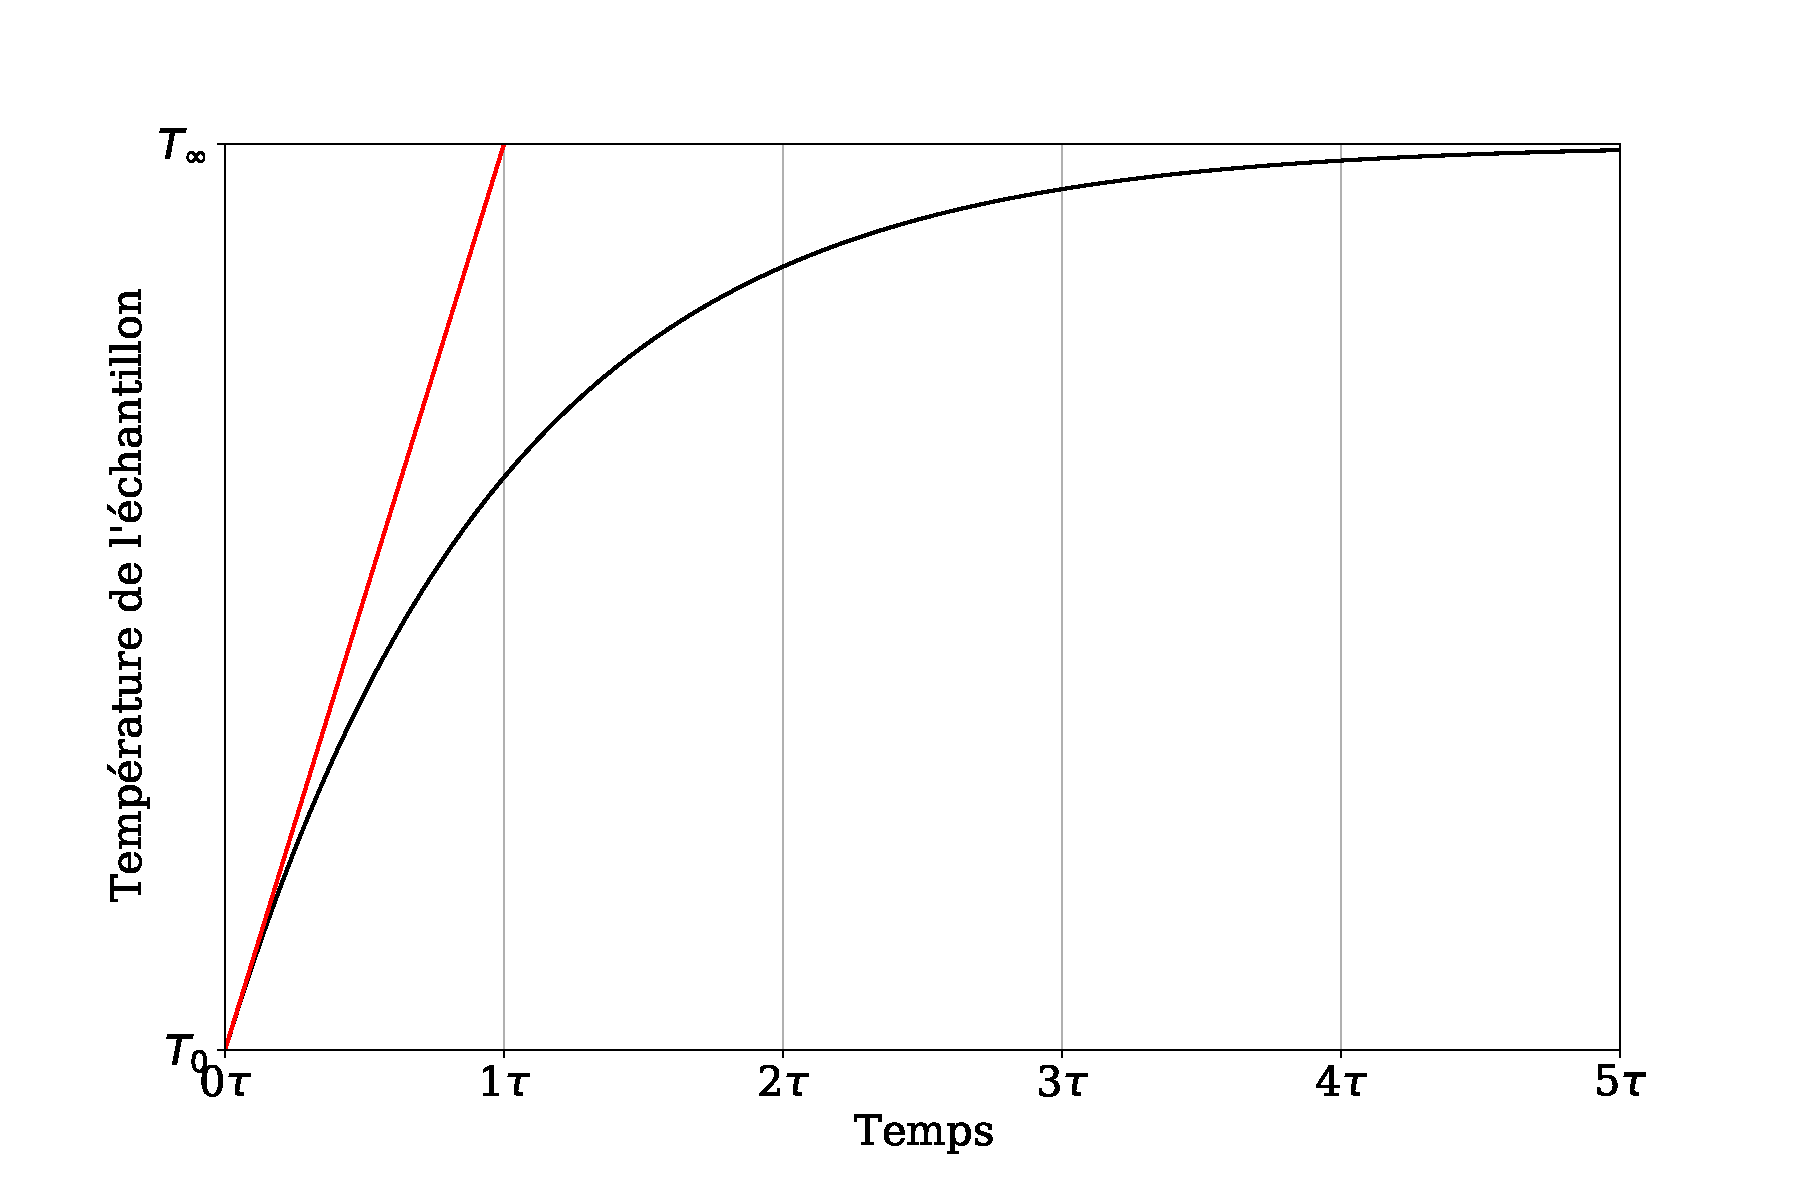
\includegraphics[height=5cm]{figures/Fig01-echauffement}}
\hspace{0.5cm}\subfloat[\label{fig:Chp1-01b}]{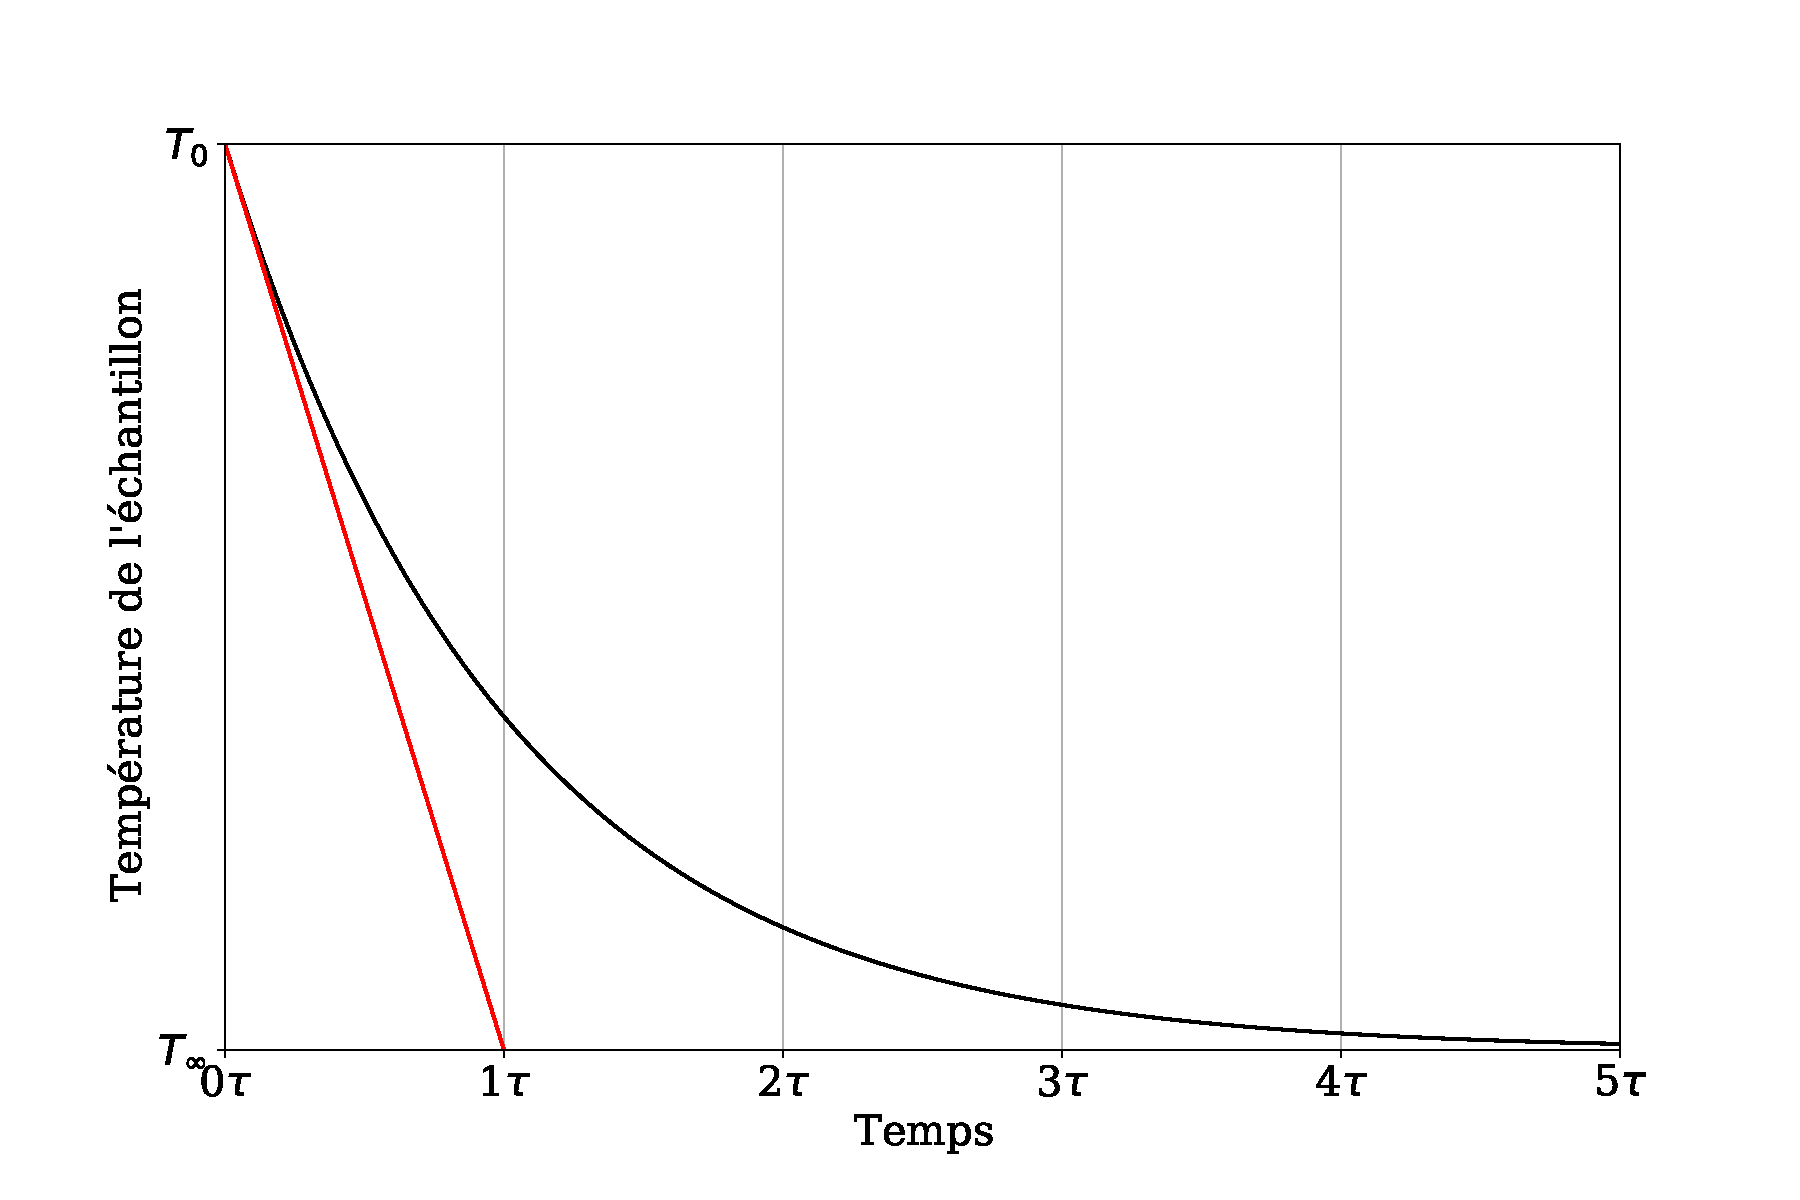
\includegraphics[height=5cm]{figures/Fig01-refroidissement}}
\end{center}
\caption{Variation de température d'un échantillon soumis à un thermostat à la température $T_\infty$, cas d'un échauffement \ref{fig:Chp1-01a} $T_\infty > T_0$ \& d'un refroidissement \ref{fig:Chp1-01b} $T_\infty < T_0$.}
\label{fig:01}
\end{figure}
}
Le refroidissement ou l'échauffement thermique d'un échantillon est d'autant plus rapide que :
\begin{itemize}
\item sa résistance thermique est petite,
\item sa capacité thermique est petite.
\end{itemize}

\subsection{Modélisation d'un refroidissement avec changement d'état}

\definition{
Le changement d'état d'un échantillon \ce{X} d'une phase $\beta$ (haute température) vers une phase $\alpha$ (basse température) :
\begin{align*}
\ce{X(\beta) ->[trans] X (\alpha)}
\end{align*}
a lieu à température constante $T^\star$, et est décrit par une équation différentielle du premier ordre : 
\begin{align*}
\frac{dn}{dt} = - \frac{T^\star - T_\infty}{R \Delta_{\beta \to \alpha} H}
\end{align*}
où $n$ est la quantité de matière de la phase $\alpha$.
}

La durée d'une transition de phase dépend : 
\begin{itemize}
\item de la différence entre la température de l'échantillon et l'extérieur ;
\item l'enthalpie de transition de phase ;
\item la résistance thermique de l'échantillon.
\end{itemize}

\subsection{Bilan}
En général, on est emmené à représenter la variation de température d'un échantillon à l'aide de portions de droites près de la température de transition de phase $T^\star$. En effet, en supposant que la durée du refroidissement soit court devant le temps caractéristique de refroidissement $t \ll \tau$, on peut alors écrire :
\begin{align*}
T(t) \approx T_\infty - (T_\infty - T_0) \frac{t}{\tau}
\end{align*}

Si l'échantillon subit une transition de phase et n'est pas soumis à phénomènes thermiques que la surfusion, on s'attend à observer l'allure suivante près de la transition  : 

\begin{figure}[H]
\centering
\begin{minipage}{0.6\textwidth}
\subfloat[\label{fig:Chp2-02a}]{
\includegraphics[height=5cm]{figures/Fig02a}}
\hspace{0.5cm}\subfloat[\label{fig:Chp2-02b}]{
\includegraphics[height=5cm]{figures/Fig02b}}
\caption{Représentation d'un refroidissement à pression constante, présentant une transition de phase d'une phase $\beta$ (HT) vers une phase $\alpha$ (BT) dans \ref{fig:Chp2-02a} une courbe de refroidissement thermique et dans \ref{fig:Chp2-02b} un diagramme pression-température.}
\label{fig:02}
\end{minipage}
\end{figure}

On observe différents points remarquables :
\begin{itemize}
\item[\textbf{A}] \ce{X} est entièrement dans la phase $\beta$ à la température $T_0$ ;
\item[\textbf{B}] le premier fragment de la phase $\alpha$ apparaît à la température $T^\star$ ;
\item[\textbf{C}] le dernier fragment de la phase $\beta$ disparaît à la température $T^\star$ ;
\item[\textbf{D}] \ce{X} est entièrement dans la phase $\alpha$ à la température $T_\infty$ ;
\end{itemize}

\section{Analyse thermique différentielle}
\subsection{Idée de la technique}	

La tête de mesure, illustrée à la Fig. \ref{fig:05}, est constituée d'une enceinte \textbf{E} de température, supposée \textbf{homogène} $T_E$ pouvant varier de manière programmée. 

\begin{minipage}{0.58\textwidth}
\centering

\includegraphics[width=\textwidth]{figures/Fig05}
\end{minipage}\hfill\begin{minipage}{0.38\textwidth}
\captionof{figure}{Montage d'un appareil d'analyse calorimétrique différentielle.}
\label{fig:05}
\end{minipage}

L'échantillon (\textbf{éch}) est contenu dans un creuset fermé, qui contient l'échantillon à étudier. Dans les mesures différentielles, un second creuset contient un corps pur de référence (\textbf{réf}), inerte thermiquement dans le domaine d'étude. La différence de température est acquis à l'aide d'un thermocouple ou d'une résistance de platine en fonction du temps.

On trouve deux programmations courante, illustrées à la Fig. \ref{fig:04a} : la rampe de température et l'isotherme.


\begin{minipage}{0.58\textwidth}
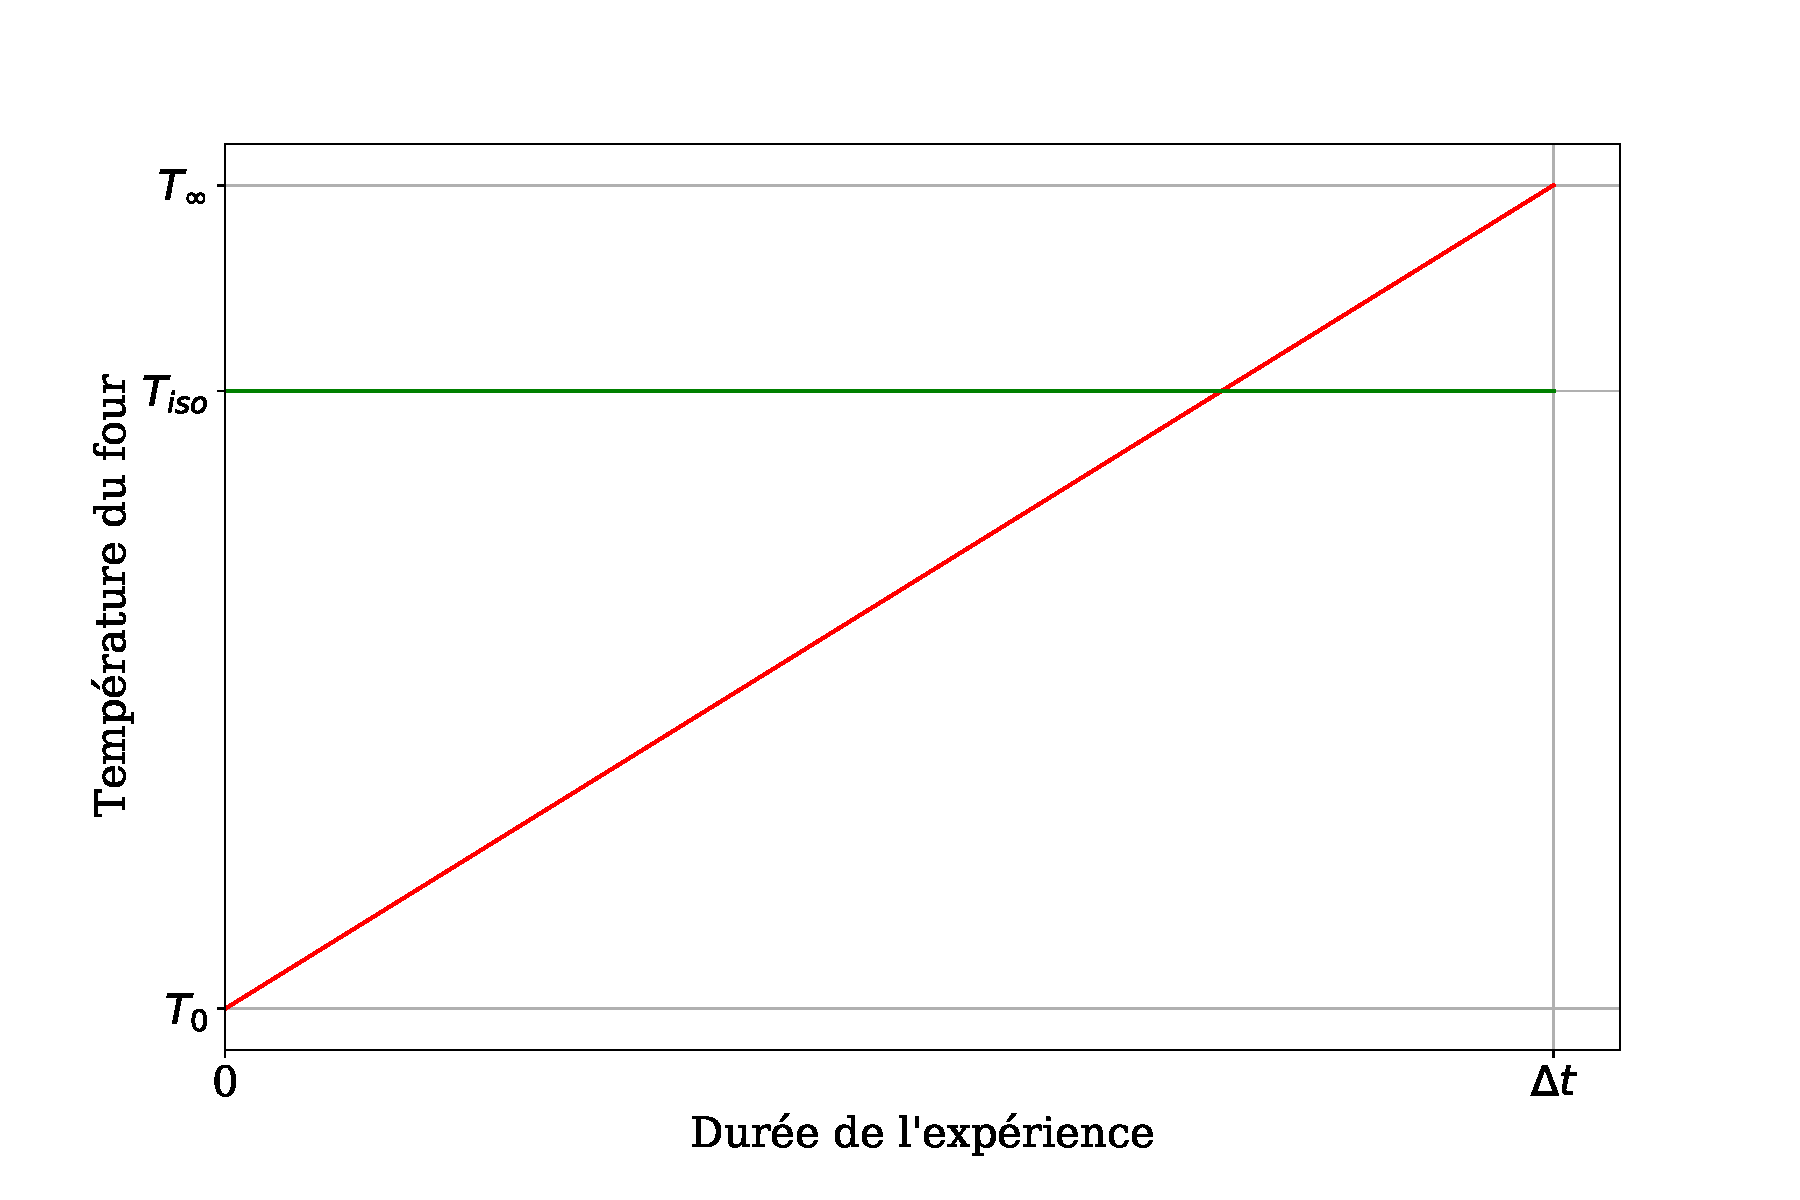
\includegraphics[width=\textwidth]{figures/Fig04a}
\end{minipage}\begin{minipage}{0.38\textwidth}
\captionof{figure}{Séquence en température, les plus courantes dans un four.}
\label{fig:04a}
[$\color{red} -$ : rampe de température, $\color{green} -$ : isotherme]
\end{minipage}

L'ensemble du montage doit être parfaitement symétrique pour que l'échantillon et la référence reçoivent la même quantité d'énergie thermique

\definition{La température du four est programmé par l'expérimentateur selon une séquence contenant, en général, une suite de rampes ($v \neq 0$) et/ou d'isothermes ($v=0$) d'équation : 
\begin{align*}
\forall t < \left\lvert \frac{T_\infty - T_0}{v} \right\rvert, \quad T_E (t) = T_0 + v \cdot t
\end{align*}
où $v$ est la vitesse de la rampe en $\si{\celsius\per\min}$.

Dans une rampe, l'expérimentateur peut contrôler : la température initiale $T_0$, la température finale $T_\infty$ et la vitesse de balayage $v$. Dans une isotherme, l'expérimentateur peut contrôler la température de l'isotherme $T_{iso}$ et la durée $\Delta t$.}

\subsection{Modélisation d'un échauffement sans changement d'état}

\definition{
Lorsqu'un expérimentateur programme une rampe de température de triplet $(T_0, T_\infty, v)$, la température d'une référence ($k=r$) et d'un échantillon idéal ($k=e$) sont décrit par l'équation différentielle linéaire du premier ordre :
\begin{align*}
\frac{dT_k}{dt}(t) + \frac{T_k (t)}{\tau_k} = \frac{T_E(t)}{\tau_k}
\end{align*}

avec $\tau_k$ le temps caractéristique associée à l'échantillon $k$ qui équivaut au produit $C_{P,k}\cdot R_k$.

Si les deux échantillons sont soumis à la même température initiale (c.-à-d. la température initiale du four) : 
\begin{align*}
T_e (0) = T_r(0) = T_0
\end{align*}
L'évolution des températures à tout instant de la rampe est donnée par l'équation :
\begin{align}
T_k(t) = \tau_k v \left[ \exp \left(- \frac{t}{\tau_k} \right) - 1 \right] + T_E (t)
\end{align}
}

\`{A} l'aide de la Fig. \ref{fig:04b}, on constate que pour un temps $t > 5 \tau_k$, l'échantillon $k$ atteint un régime \textbf{permanent} et \textbf{non stationnaire} : 

\begin{align*}
\forall t \gg \tau_r, T_r (t) &= T_E(t) - \tau_r v \\
\forall t \gg \tau_e, T_e (t) &= T_E(t) - \tau_e v
\end{align*}

A chaque instant, la température de l'échantillon et la référence ont un retard qui augmente avec : 
\begin{itemize}
\item la vitesse de balayage en température ;
\item la capacité calorifique de chaque échantillon ; 
\item la résistance thermique de chaque échantillon.
\end{itemize}


\begin{minipage}{0.58\textwidth}
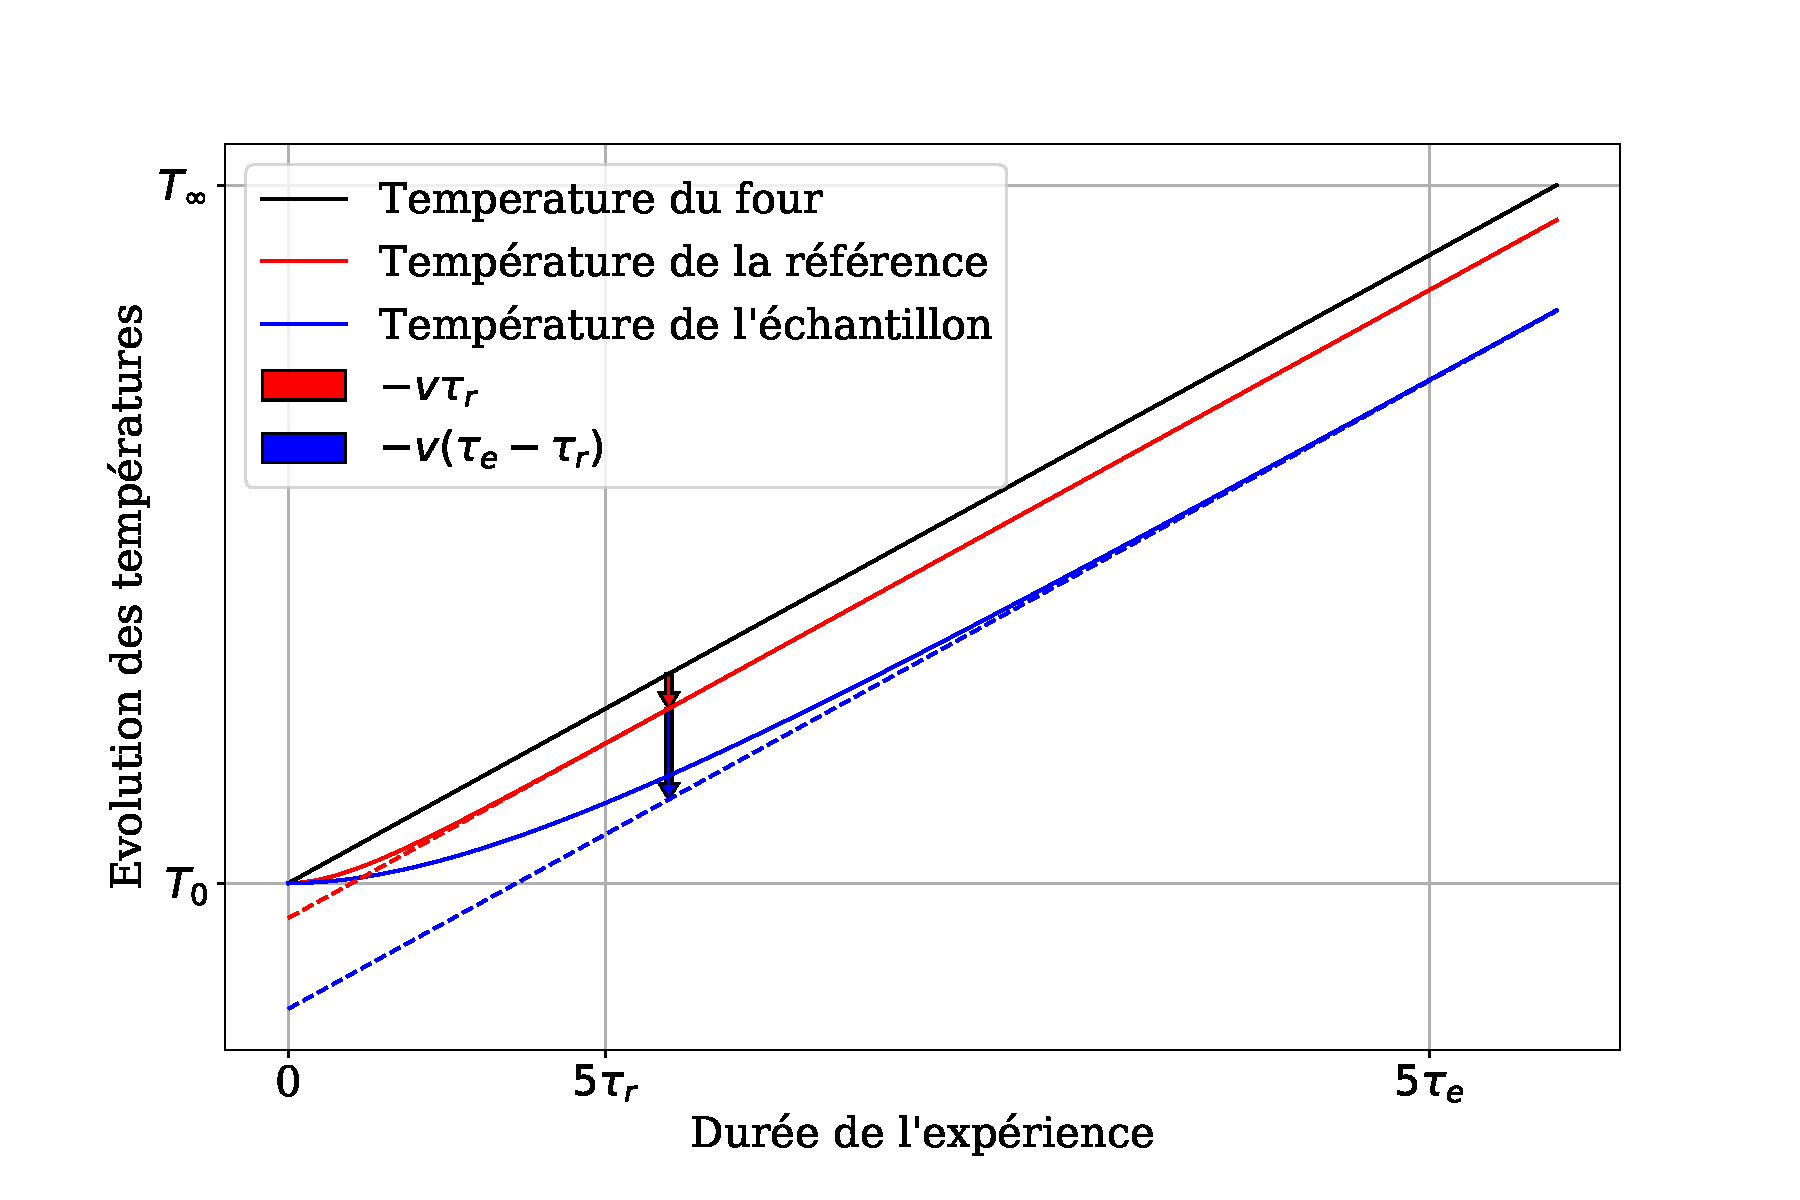
\includegraphics[width=\textwidth]{figures/Fig04b}
\end{minipage}\begin{minipage}{0.38\textwidth}
\captionof{figure}{Réponse en température de l'échantillon et de la référence, en considérant que $\tau_r < \tau_e$, à l'élévation en température du four de l'ATD.}
\label{fig:04b}
\end{minipage}

En calorimétrie différentielle, on s'intéresse à la différence de température entre l'échantillon et la référence : 
\begin{align*}
\forall t \gg \max \left\{ \tau_r, \tau_e \right\},  \Delta T (t) &= T_e (t) - T_r (t) \\
&= -v (\tau_e - \tau_r)
\end{align*}

Cette grandeur constitue la nouvelle \textbf{ligne de base} du signal ATD comme représentée à la Fig. \ref{fig:04d}.

\begin{minipage}{0.58\textwidth}
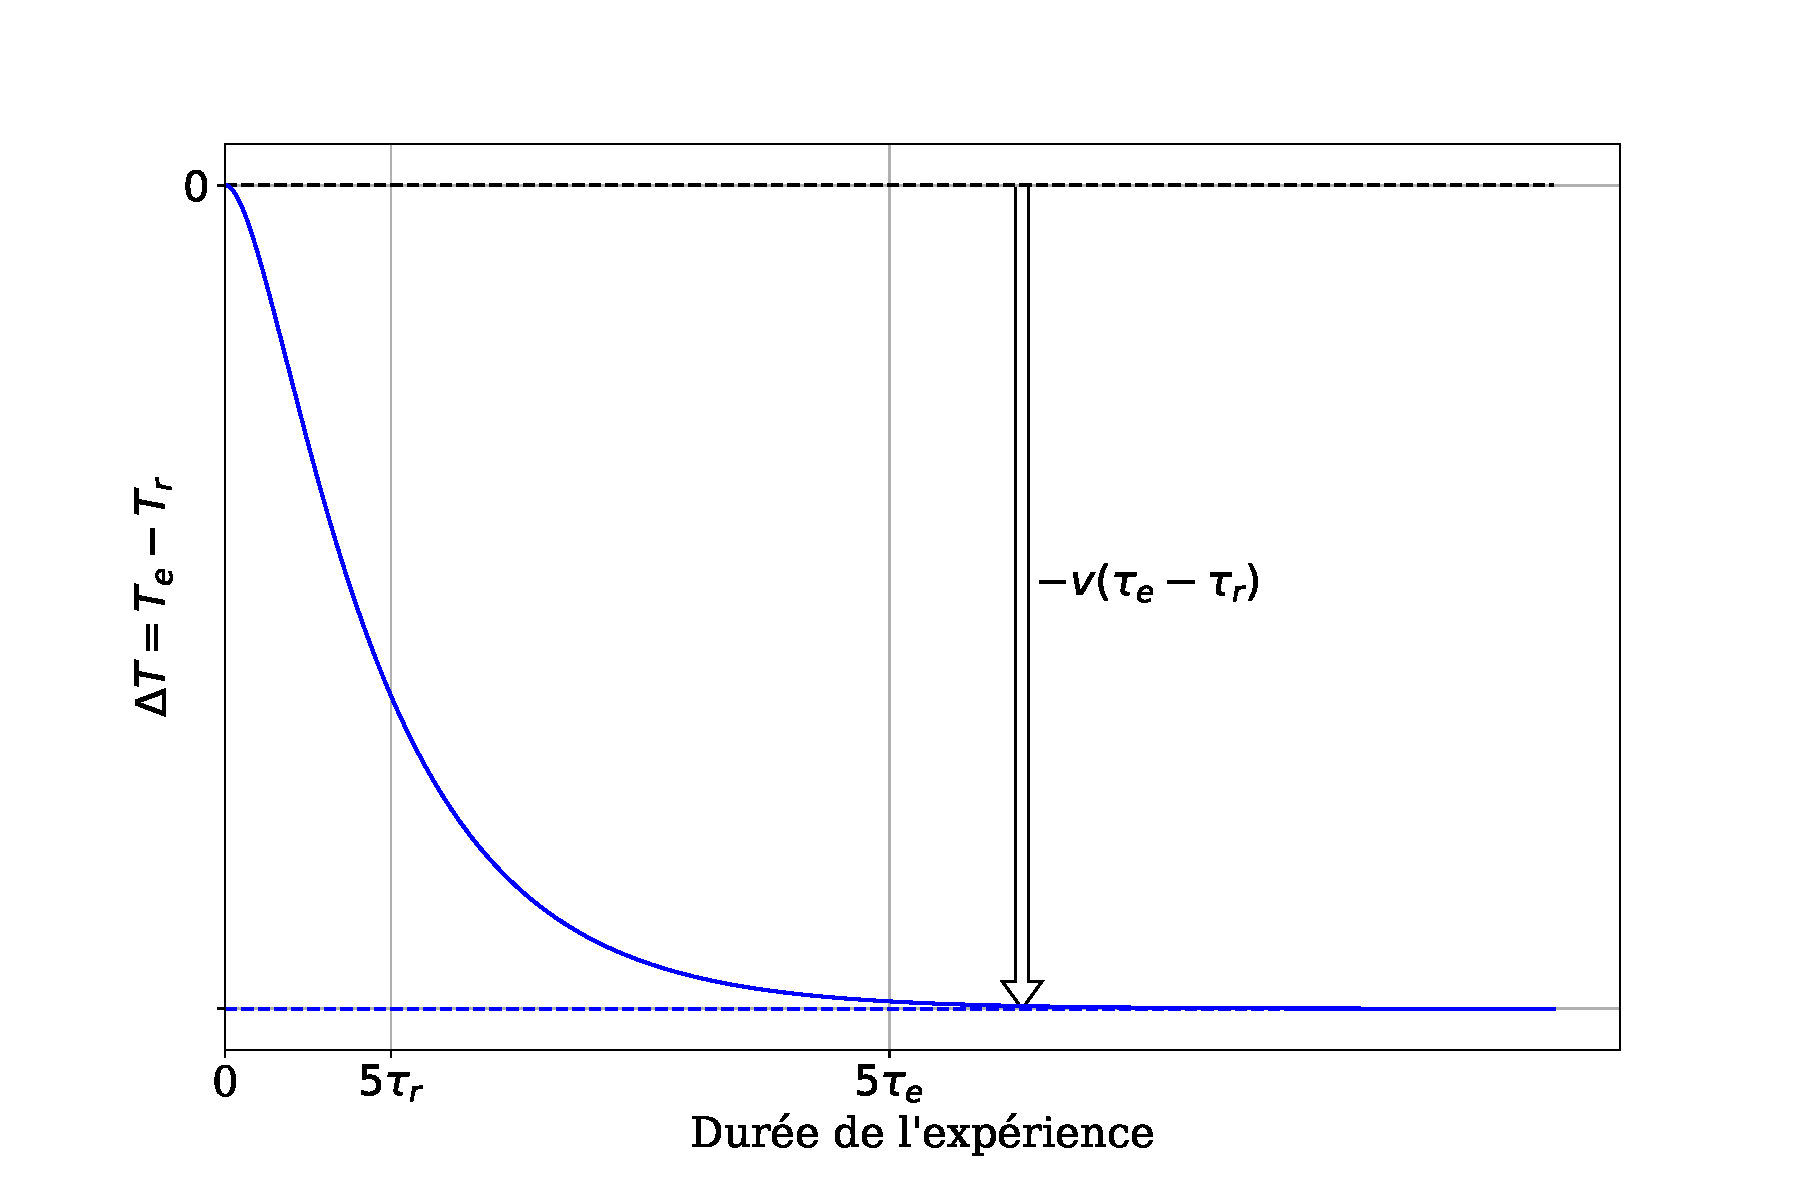
\includegraphics[width=\textwidth]{figures/Fig04d}
\end{minipage}\begin{minipage}{0.38\textwidth}
\captionof{figure}{Après un temps d'induction de l'ordre de $5 \tau_e$, la ligne de base du signal calorimétrique est établie.}
\label{fig:04d}
[$\color{red} -$ : rampe de température, $\color{green} -$ : isotherme]
\end{minipage}

\example{
Commenter le déplacement de ligne de base lors de la fusion et de l'évaporation de l'eau
\begin{figure}[H]
\centering
\begin{minipage}{0.8\textwidth}
\subfloat[\label{fig:Chp2-07a}]{
\includegraphics[height=4.5cm]{figures/Fig07a}}
\hspace{0.5cm}\subfloat[\label{fig:Chp2-07b}]{
\includegraphics[height=4.5cm]{figures/Fig07b}}
\captionof{figure}{Zoom du pic de fusion \ref{fig:Chp2-07a} et du pic d'évaporation \ref{fig:Chp2-07b} de l'eau à une vitesse de balayage constante de \SI{10}{\celsius\per\min}}
[l'intégration se fait en utilisant une intégrale tangentielle ou une intégrale horizontale]
\label{fig:02}
\end{minipage}
\end{figure}
}

\subsection{Modélisation d'un échauffement avec changement d'état}

Prenons un échantillon solide idéal, subissant une fusion, c.-à-d. que sa température de fusion $T^\star$ est inclue dans l'intervalle $[T_0, T_\infty]$. Si on considère que le solide et le liquide ont une capacité thermique similaire, on s'attend à ce que l'échantillon et la référence réponde comme représenté à la Fig. \ref{fig:04c}.

\begin{minipage}{0.58\textwidth}
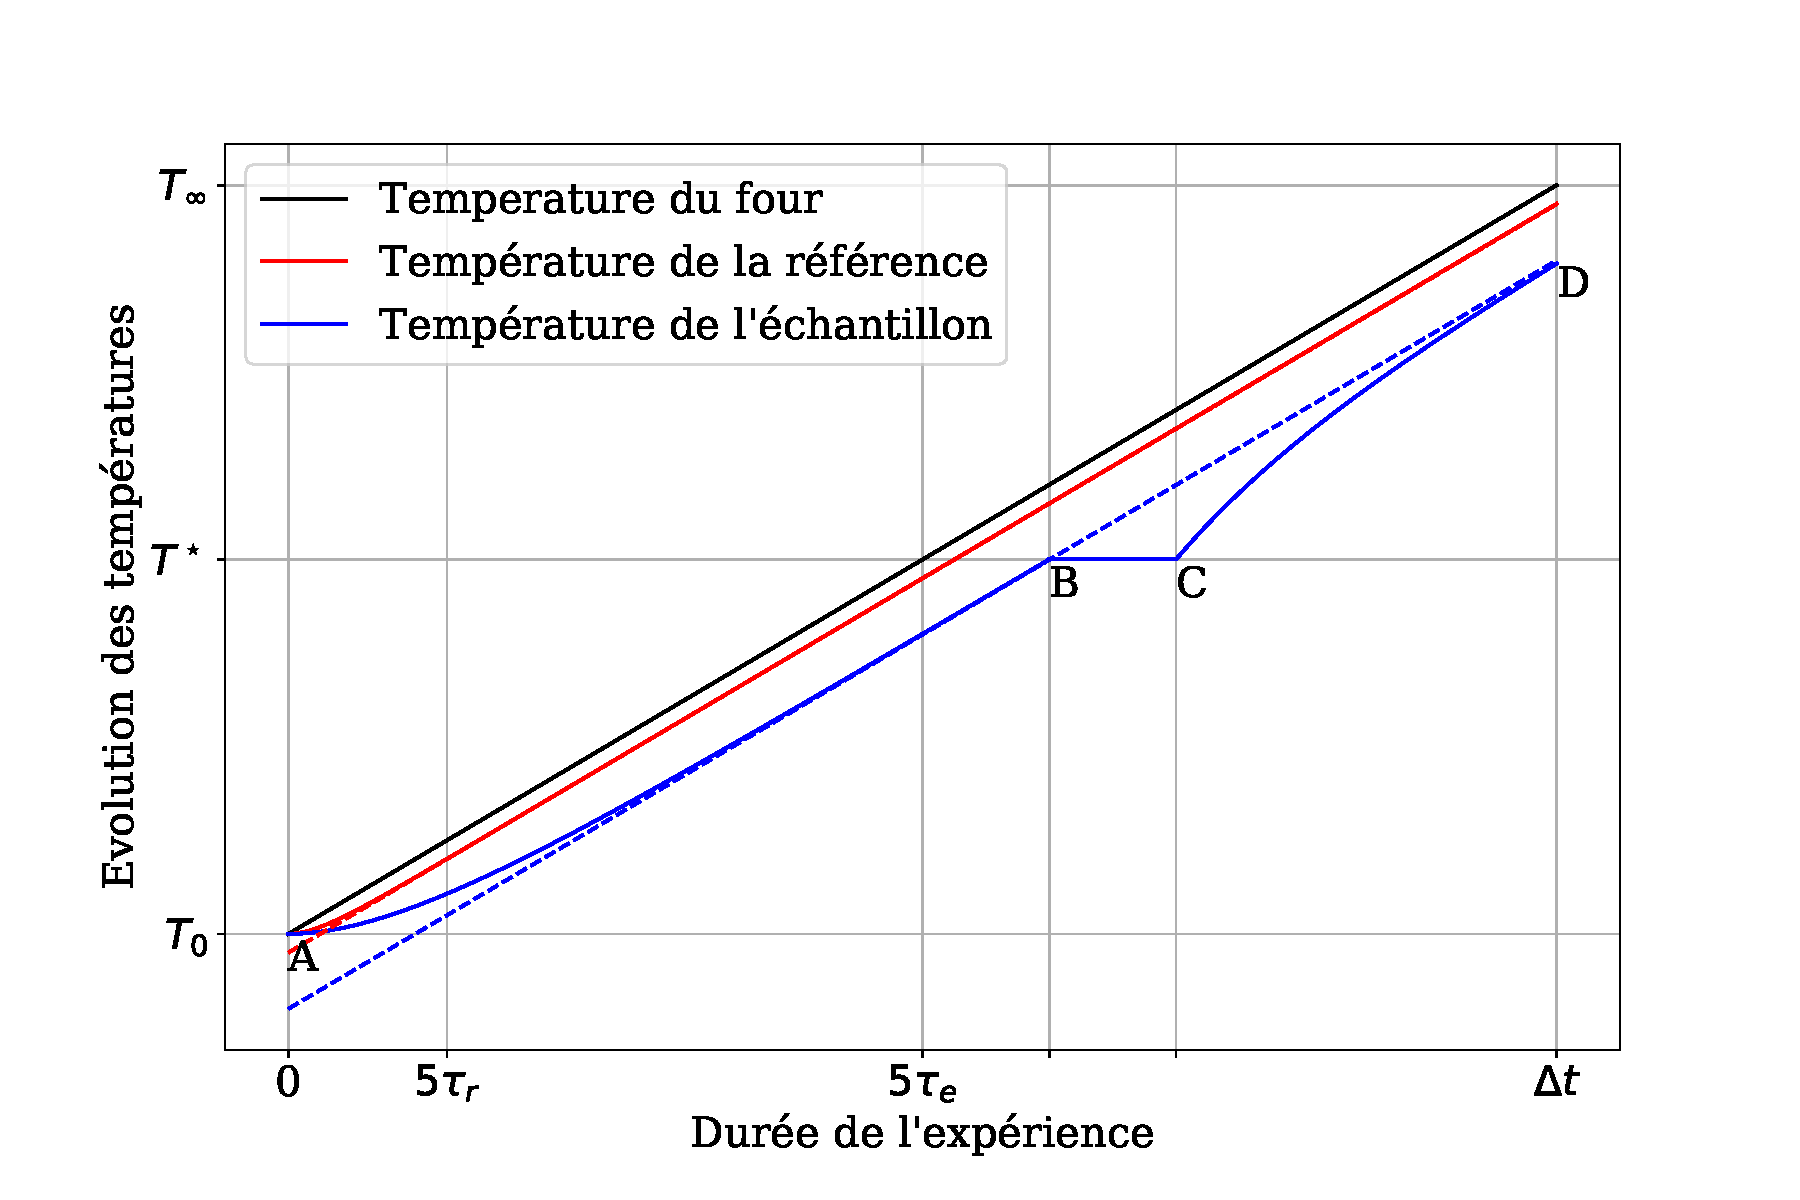
\includegraphics[width=\textwidth]{figures/Fig04c}
\end{minipage}\begin{minipage}{0.38\textwidth}
\captionof{figure}{Réponse en température de l'échantillon, présentant une fusion, et de la référence, en considérant que $\tau_r < \tau_e$, à l'élévation en température du four de l'ATD.}
\label{fig:04c}
\end{minipage}

On observe 3 étapes : 
\begin{itemize}
\item[\textbf{AB}] échauffement du solide ;
\item[\textbf{BC}] fusion du solide ;
\item[\textbf{BC}] échauffement du liquide ;
\end{itemize}

Dans un corps pur idéal, la fusion a lieu à un palier de température. Lorsque le processus est terminé, il apparaît un nouveau régime \textbf{transitoire} dû au retard en température pris par l'échantillon par rapport au four.

Quand on regarde la différence de température entre l'échantillon et la référence, toutes les "anomalies thermiques", processus différent d'un échauffement ou d'un refroidissement, vont conduire à l'apparition d'un pic comme représenté à la Fig. \ref{fig:04e}.

\begin{minipage}{0.58\textwidth}
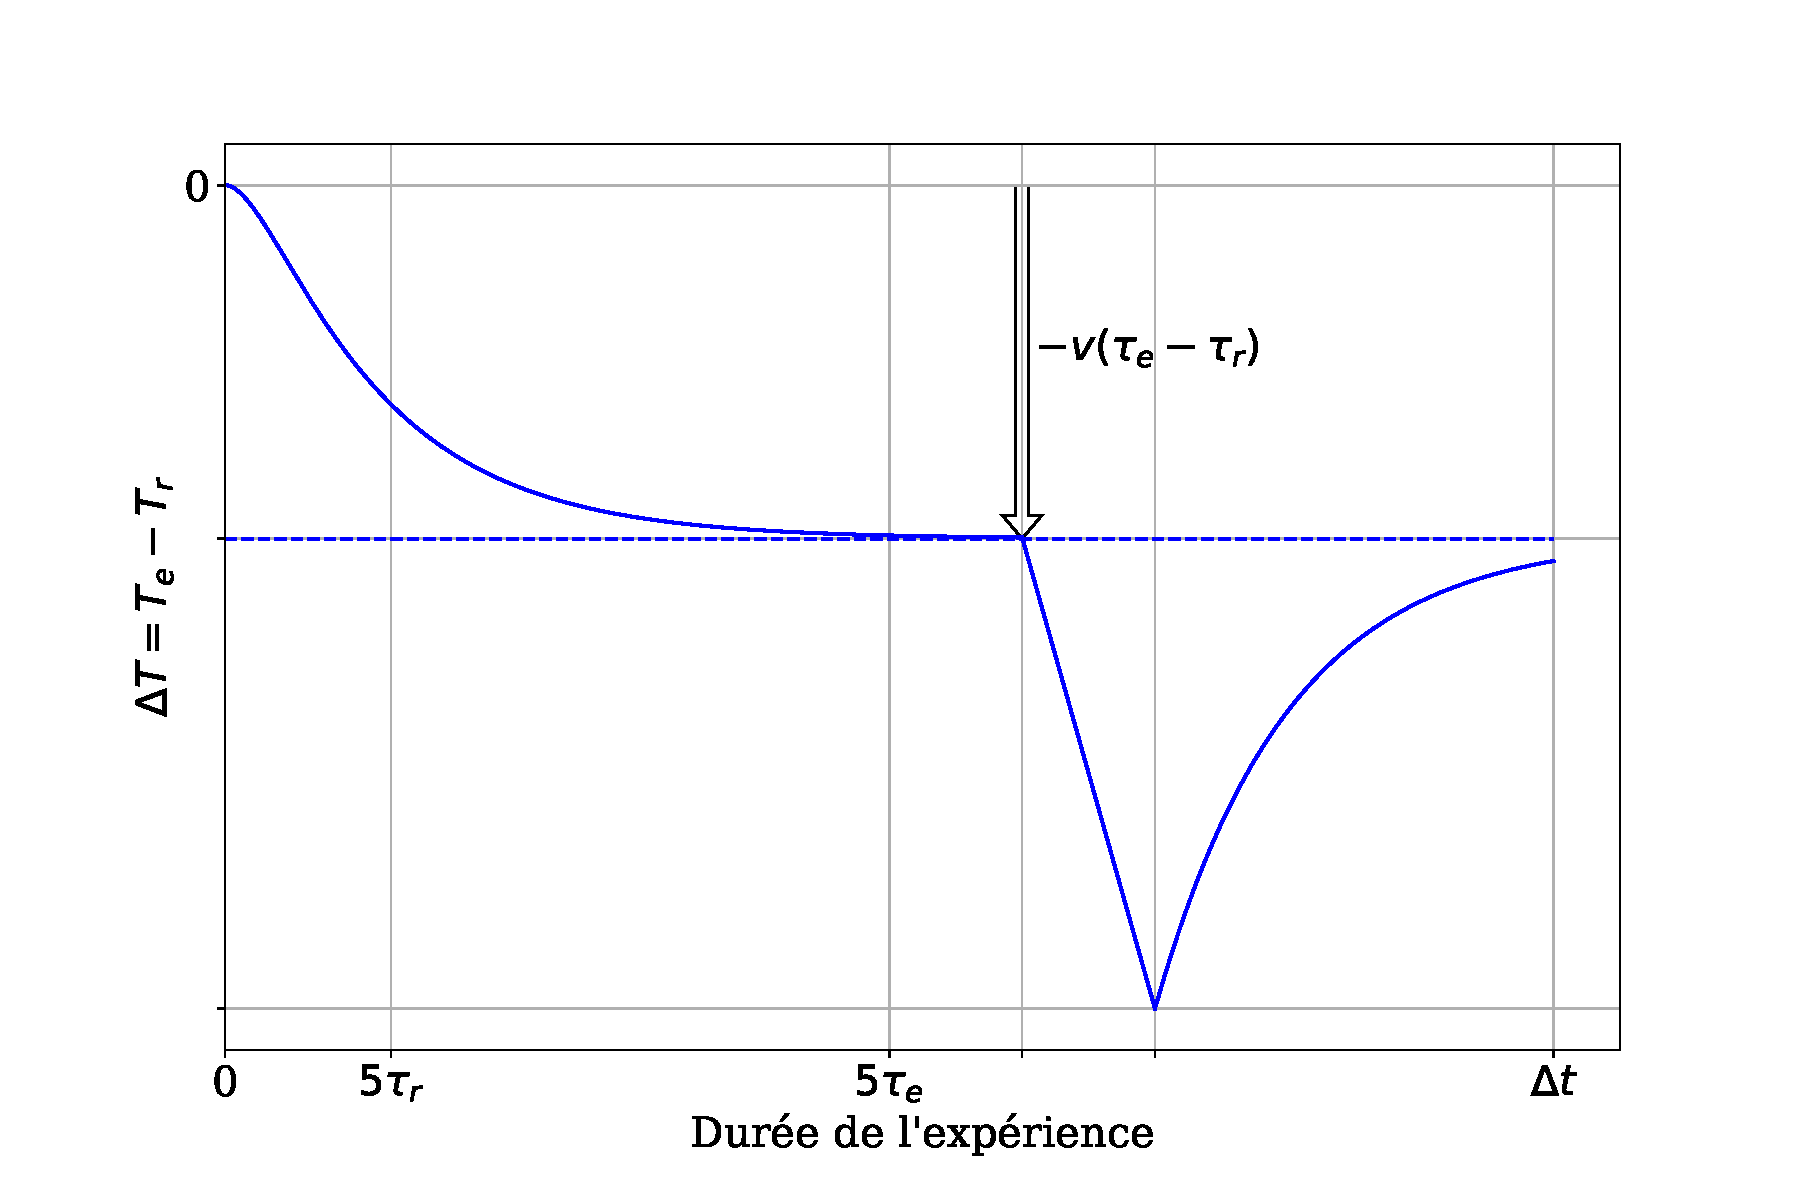
\includegraphics[width=\textwidth]{figures/Fig04e}
\end{minipage}\begin{minipage}{0.38\textwidth}
\captionof{figure}{Dans un signal ATD, une "anomalie thermique", conduit à l'apparition d'un pic (ici endothermique).}\label{fig:04e}
\label{fig:04e}
\end{minipage}

\definition{
Dans la réalité, la forme d'un pic "ATD" est beaucoup moins anguleux que la modélisation idéale proposée. Plusieurs phénomènes ne sont pas pris en compte : 
\begin{enumerate}
\item arrondi en début de palier traduit la présence d'une impureté,
\item le creuset, contenant l'échantillon, continue de s'échauffer pendant la transition de phase (le palier n'est pas parfaitement horizontal).
\end{enumerate}
}

\example{
Commenter l'allure des pics de DSC suivants :
\begin{figure}[H]
\centering
\begin{minipage}{0.8\textwidth}
\subfloat[\label{fig:Chp2-06a}]{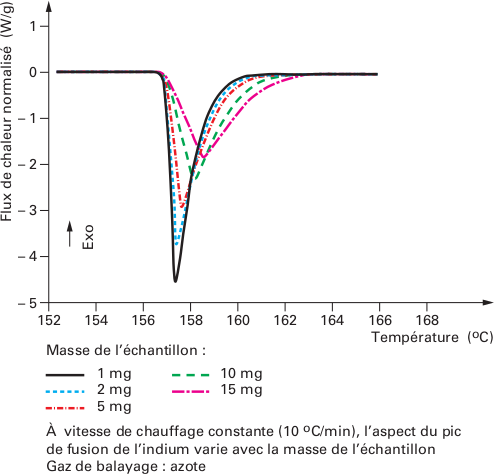
\includegraphics[height=6cm]{figures/Fig06a}}
\hspace{0.5cm}\subfloat[\label{fig:Chp2-06b}]{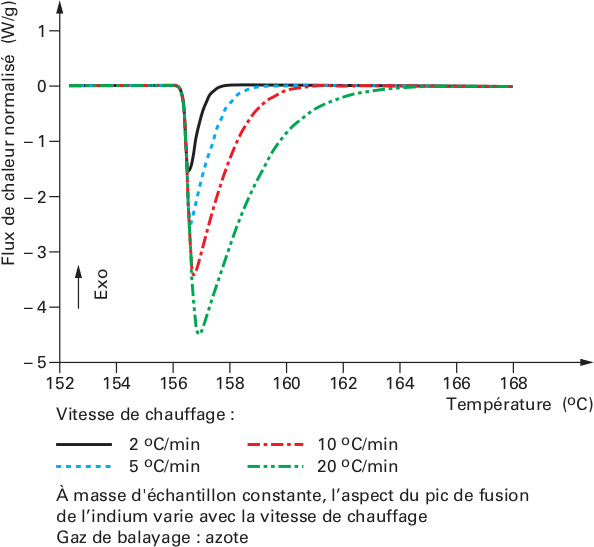
\includegraphics[height=6cm]{figures/Fig06b}}
\caption{\'{E}tude de l'influence de la masse et de la vitesse de balayage sur le pic de fusion de l'indium}
\label{fig:02}
\end{minipage}
\end{figure}
}

\subsection{Relation entre le signal calorimétrique et l'enthalpie}

En ATD, on cherche en général à déterminer les enthalpies de transition associées aux anomalies thermiques. 

\definition{L'enthalpie, associée aux anomalies thermiques, est proportionelle à la surface du pic du signal calorimétrique (corrigée de sa ligne de base) : 

\begin{align*}
\Delta H &= K \int \Delta \bar{T} (t) dt \\
&= K \int \bar{T}_e (t) - \bar{T}_r (t) dt \\
&= K \cdot S
\end{align*}

avec $\bar{T}$ la température suite à la correction de ligne de base. 

Le c{\oe}fficient $K$ ne peut être déterminé que par un \textbf{étalonnage} préalable de la machine.
}

Il est impossible de déterminer théoriquement le paramètre $K$, qui dépend de la géométrie de échantillons, de la symétrie dans l'enceinte, de la conductivité thermique des échantillons, des constantes de temps$\ldots$

Toute estimation d'une enthalpie de transformation nécessite de prendre en compte la masse ou la quantité de matière de l'échantillon : 
\begin{align*}
\Delta_{trans} H = \frac{\Delta H}{\text{masse ou quantité de matière de l'échantillon}}
\end{align*}

En général, on cherche dans un signal calorimétrique à indiquer une convention permettant de distinguer les anomalies thermiques au-dessus de la ligne de base, et celles en-dessous. 

\definition{On doit donc indiquer sur son thermogramme, si un pic, associée à une anomalie thermique, au-dessus de la ligne de base correspond à un processus \textbf{EXO} (exothermique) /\textbf{ENDO} (endothermique).}

Malgré un étalonnage soigné, l'ATD reste une technique assez peu reproductible. Elle reste toutefois la seule technique d'analyse pour les hautes températures ($800-2400 ~ \si{\celsius}$)

\section{Differential Scanning Calorimetry (DSC)}
La DSC, développée par la société PerkinElmer, est une technologie de choix pour l'étude des phénomènes thermiques entre -160 et \SI{800}{\celsius}.

La principale différence avec l'ATD est que l'on mesure, en plus de la température de l'échantillon $T_e (t)$ et de la température de la référence $T_r (t)$, le flux de chaleur \textbf{émi} par l'échantillon.

\subsection{Modélisation idéale : DSC conventionnelle, mode $T_1$}
Les paramètres mesurés forment un quadruplet : ($\Phi_e$, $\Phi_r$, $T_e$, $T_r$)

Si on suppose que le four a une température uniforme $T_E$ et que l'échantillon et la référence ont la même résistance thermique $R \approx R_e \approx R_r$, la différence de flux thermique est proportionnelle à la différence de température : 
\begin{align}
\Delta \Phi &= \Phi_e - \Phi_r = \left( \frac{T_e - T_E}{R_e}\right) - \left( \frac{T_r - T_E}{R_e}\right) \\
&= \frac{T_e - T_r}{R}
\end{align}

\definition{
En théorie, la mesure de la différence de flux thermique reçu de l'échantillon par rapport à la référence par la DSC, permet de retrouver les phénomènes thermiques modélisés dans l'ATD.
}

En réalité, dans la DSC, les principales divergences à la relation précédente sont d'ordre "machine" : 
\begin{itemize}
\item $\Delta \Phi$ ne vaut pas 0 même en l'absence de creuset, à cause des différences infinitésimal d'usinage des porte-échantillons, capteurs$\ldots$
%0.00127 mm de différence conduit à une différence de résistance thermique de 1%
\item On ne prend pas en compte la différence de résistance thermique entre le couple échantillon-four et le couple référence-four ;
\item la capacité thermique du creuset et du capteur est ignorée ;
\item la température mesurée est supposée égale à celle de l'échantillon contenu dans le creuset ,
\item les fuites thermiques de l'enceinte.
\end{itemize}

L'ensemble de ces "défauts", ont pour conséquence :
\begin{itemize}
\item de briser la planéité de la ligne de base en la rendant courbe,
\item la rampe de température n'est pas strictement identique en l'échantillon et la référence
\end{itemize}
Par conséquent, le premier (resp. dernier) point résulte en une perte de sensibilité (resp. resolution).

\subsection{Modélisation élaborée : DSC avancée, mode $T_4$}

La plupart des capteurs actuels mesurent la température entre plus de deux points, ce qui offre la possibilité d'élaborer des modèles thermiques plus complexes prenant en compte les sources d'erreurs introduites par les hypothèses simplificatrices de la section précédente.

\begin{center}
\begin{minipage}{0.48\textwidth}
\centering

\includegraphics[width=0.5\textwidth]{figures/Fig08}
\end{minipage}\hfill\begin{minipage}{0.48\textwidth}
\captionof{figure}{Capteur de la marque TA Instrument mesurant en trois points (=mode $T_4$)}
\end{minipage}
\end{center}


Les paramètres mesurés forment un quintuplet : $(\Phi_e, \Phi_r, T_e, T_r, T_0)$. On ajoute un point de mesure, appelé point 0, à équidistance des deux échantillons et de la référence où sera mesuré la température $T_0$.

Par conséquent, on s'intéresse à trois différences mesurables : 
\begin{itemize}
\item la différence du flux d'énergie reçu par la machine : 
\begin{align*}
\color{red} \Delta \Phi = \Phi_e - \Phi_r
\end{align*}
\item la différence de température entre l'échantillon et la référence : 
\begin{align*}
\color{blue} \Delta T = T_e - T_r
\end{align*}
\item la différence de température entre l'échantillon et le point 0 : 
\begin{align*}
\color{green} \Delta T_0 = T_e - T_0
\end{align*}
\end{itemize}

Un développement mathématique de la relation permet de décomposer la différence de flux thermique reçu par la machine en 4 composantes : 
\begin{align*}
{\color{red} \Delta \Phi} = \underbrace{- \frac{{\color{blue} \Delta T}}{R_r}}_{(1)} + \underbrace{\left( \frac{1}{R_r} - \frac{1}{R_e} \right) {\color{green} \Delta T_0}}_{(2)} \underbrace{- C_r \frac{d {\color{blue} \Delta T}}{dt}}_{(3)} + \underbrace{(C_r - C_e) \frac{d T_e}{dt}}_{(4)}
\end{align*}

Chacune des composants prend en compte un phénomène différence : 
\begin{enumerate}
\item Flux principal dû aux anomalies thermiques ;
\item Différence de résistance thermique entre les deux échantillons ;
\item Différence de vitesse de chauffe entre les deux échantillons ;
\item Différence de capacité thermique entre les deux échantillons.
\end{enumerate}

Dans ce type de modèle, l'expérimentateur réalise un étalonnage permettant de paramétriser l'équation précédente.

\end{document}
